\documentclass[../ClassicThesis.tex]{subfiles}
\begin{document}

%************************************************
\chapter{Classifiers}\label{ch:classifiers}
\newcommand{\TODO}[1]{\textcolor{red}{\\ \textbf{TODO:} #1 \\}}
%************************************************

\section{Classifiying idea}
\TODO{From what paper did we take this? and CGAl etc.}
\paragraph{What is it usually used for? - pointclouds... which points do we intend to take for the algorithm?}
\section{RANSAC - Random Sample Consensus}
The RANSAC-approach firstly chooses a defined number of random points. These points are a minimal set from the point data and its number is defined by the shape which is being classified.\\
On the basis each of these minimal sets a candidate shape is generated and tested against all points in the data set. The candidate gets a score which tells how well the randomly chosen points represent the shape. This score can result from counting the points which lie within the candidate.\\
Based on this score a best model is saved or overwritten after several candidate attempts.
\section{Primitives}
In order to classify primitives a minimum number of points has to be defined which enable a reconstruction of the shape.
\subsection{Plane}
The minimal set for a plane are three points \{p1, p2, p3\} because three points uniquely identify a plane.\\
Once a plane candidate has been found it is necessary to check its plausibility. The deviations of the plane normal to the according point normals of p1, p2 and p3 should be less than an angle $\alpha$.\\
\*\\
After the detection of a best model it may be necessary to refit the candidate to all its inliers. We use the Least Squares method [\TODO{cite here}]. We are aware that this method can only compute planes where its z-values are dependent on the x- and y-values which is not the case the the plane is perpendicular to the x-y-plane. Therefore we ignore planes to which this applies. Another possibility would be to work with eigenvectors where this would not be an issue.\\
When using the least squares method the problem can be transformed into an equation of the form Ax = b. Where A is a matrix consisting of the sum of all x values of the points, y values, x times y and x squared and y squared. \\
See http://www.geometrictools.com/Documentation/LeastSquaresFitting.pdf for a detailed explanation.
\subsection{cylinder}
The minimal set for a cylinder are two points \{p1, p2\}. Those points are assumed to lie on the shell of the cylinder. The axis can be calculated by calculating the crossproduct of their normals. Based on the axis a projection plane is formed which is perpendicular to the axis. The two lines l1 = p1 + t*n1 and l2 = p2 + t*n2 are projected onto this plane and should have an intersection. If they do not intersect the candidate is invalid. Otherwise, the intersectionpoint is marked as the center of the cylinder-candidate. The radius is the mean value of the distance of both points to the center on the axis.\\
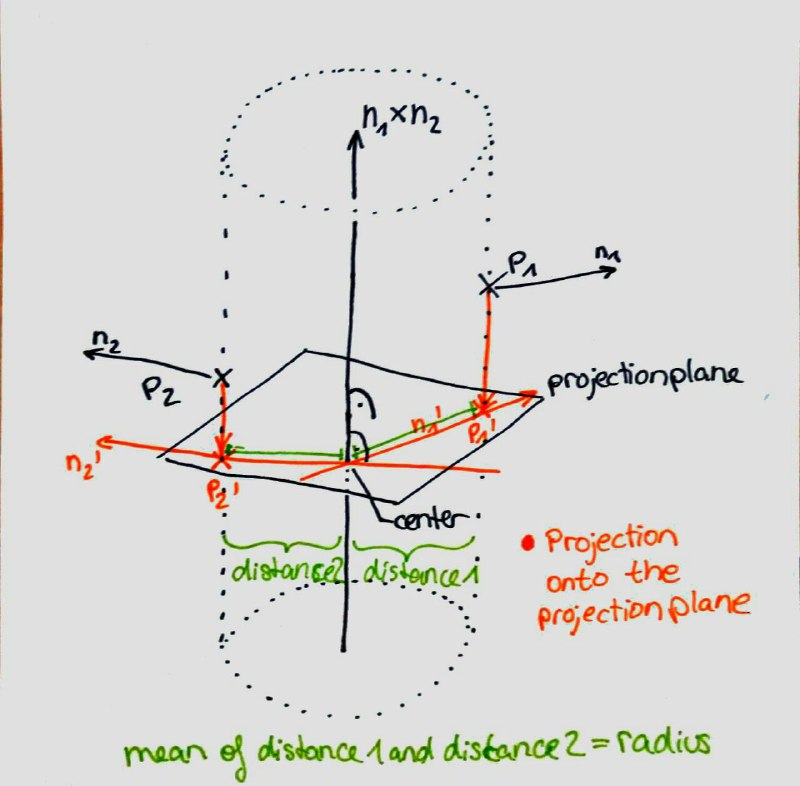
\includegraphics[width=\columnwidth]{Images/10-classifiers-cylinderClassification.jpg}
After a valid candidate has been formed we have to check the plausibility. For this we look for three indication. Firstly, the randomly chosen points p1 and p2 should not be the same, secondly, the calculated radius has to be larger than zero and lastly, the distances of the two points to the center should not exceed an epsilon value $\epsilon$.
\subsection{Prism - Dimitri}
\subsection{Other primitives}
\section{Problems with non-pointcloud input}
In our usecase we do not have a pointcloud as input. Instead we operate on the much fewer points in a polygon mesh.\\
This has large influences on the threshold values that are used. The values taken from CGAL almost never achieved the desired results. We tried finding new values for any model which turned out to be infeasible. Therefore we tried adjusting the thresholds based on the number of vertices in the mesh or the volume of the bounding box. We have not encountered a working combination yet. This is a problem that needs to be tackled in future work.
\end{document}